%%%%%%%%%%%%%%%%%%%%%%%%%%%%%%%%%%%%%%%%%%%%%%%%%%%%%%%%%
%                          导言区                        %
%%%%%%%%%%%%%%%%%%%%%%%%%%%%%%%%%%%%%%%%%%%%%%%%%%%%%%%%%
\documentclass[13pt]{ctexart} % 文档类
% 基础样式
\usepackage{geometry} % 设置页面
\renewcommand{\figurename}{Figure} % 设置标题 重命名为英文
\renewcommand{\tablename}{Table}
\renewcommand{\contentsname}{Contents}
\usepackage{changepage} % 设置摘要页缩减
\usepackage{fontspec} % 便于修改字体
\usepackage{fancyhdr} % 设置页眉页脚
\pagestyle{fancy} % 清空页眉页脚
\usepackage{lastpage}
\usepackage{titlesec} % 设置修改默认的section标题样式
\titleformat*{\section}{\LARGE\bfseries}
\titleformat*{\subsection}{\Large\bfseries}
\titleformat*{\subsubsection}{\Large\bfseries}
\usepackage[section]{placeins} % 新增: 浮动体不越过section
% 浮动体样式
\usepackage[shortlabels]{enumitem} % 设置列表缩进
\usepackage{booktabs} % 三线表宏包
\usepackage{array} % 设置表格的列格式
\usepackage{graphicx} % 插图片
\graphicspath{{C:/Users/zheng/Desktop/mcm-2021/mcmdocs/figs/}}
% 数学样式
\usepackage{amsmath} % 使用数学宏包
\usepackage{amsfonts} % 使用数学字体
% bib样式
\usepackage{etoolbox} % 设置参考文献不输出默认名
\usepackage{newtxtext}
\patchcmd{\thebibliography}{\section*{\refname}}{}{}{} % 引入网站作为参考文献
\usepackage[]{hyperref} % 设置引用且末尾不显示文档名
% 代码样式
\usepackage{url} % 设置等宽的代码字体
%%\setmonofont{IBM Plex Mono}
%% 建议这个,但我系统没这个字体,且懒得折腾了
%%windows用户请
\setmonofont{Courier New}
% 颜色
\usepackage{xcolor} % 代码高亮方案宏包
\usepackage{listings}
\definecolor{CPPLight}  {HTML} {686868}
\definecolor{CPPSteel}  {HTML} {888888}
\definecolor{CPPDark}   {HTML} {262626}
\definecolor{CPPBlue}   {HTML} {4172A3}
\definecolor{CPPGreen}  {HTML} {487818}
\definecolor{CPPBrown}  {HTML} {A07040}
\definecolor{CPPRed}    {HTML} {AD4D3A}
\definecolor{CPPViolet} {HTML} {7040A0}
\definecolor{CPPGray}   {HTML} {B8B8B8}
\lstset{
	basicstyle=\ttfamily,
	breaklines=true,
	framextopmargin=50pt,
	frame=bottomline,
	columns=fixed,
    %numbers=left,                                       % 在左侧显示行号
	frame=none,                                          % 不显示背景边框
	backgroundcolor=\color[RGB]{255,255,255},            % 设定背景颜色
	keywordstyle=\color[RGB]{40,40,255},                 % 设定关键字颜色
	numberstyle=\footnotesize\color{darkgray},           % 设定行号格式
	commentstyle=\itshape\color[RGB]{0,96,96},           % 设置代码注释的格式
	stringstyle=\slshape\color[RGB]{128,0,0},            % 设置字符串格式
	showstringspaces=false,                              % 不显示字符串中的空格
	language=python,                                     % 设置语言
	morekeywords={alignas,continute,friend,register,true,alignof,decltype,goto,
		reinterpret_cast,try,asm,defult,if,return,typedef,auto,delete,inline,short,
		typeid,bool,do,int,signed,typename,break,double,long,sizeof,union,case,
		dynamic_cast,mutable,static,unsigned,catch,else,namespace,static_assert,using,
		char,enum,new,static_cast,virtual,char16_t,char32_t,explict,noexcept,struct,
		void,export,nullptr,switch,volatile,class,extern,operator,template,wchar_t,
		const,false,private,this,while,constexpr,float,protected,thread_local,
		const_cast,for,public,throw,std},
	emph={map,set,multimap,multiset,unordered_map,unordered_set,numpy,graph,path,append,extend,
		unordered_multiset,unordered_multimap,vector,string,list,deque,
		array,stack,forwared_list,iostream,memory,shared_ptr,unique_ptr,
		random,bitset,ostream,istream,cout,cin,endl,move,default_random_engine,
		uniform_int_distribution,iterator,algorithm,functional,bing,numeric,},
	emphstyle=\color{CPPViolet},
}

%%%%%%%%%%%%%%%%%%%%%%%%%%%%%%%%%%%%%%%%%%%%%%%%%%%%%%%%%
%                         正文区                         %
%%%%%%%%%%%%%%%%%%%%%%%%%%%%%%%%%%%%%%%%%%%%%%%%%%%%%%%%%
\begin{document}
%%%%%%%%%%%%%%%%%%%%%%%%%%扉页%%%%%%%%%%%%%%%%%%%%%%%%%%
\newgeometry{left=1in,right=0.75in,top=1in,bottom=1in}
% 第一页的字体为times new roman
\setmainfont{Times New Roman}
\thispagestyle{empty}
% 扉页抬头

\vspace*{-16ex}
\centerline{\begin{tabular}{*3{c}}
        \parbox[t]{0.3\linewidth}{
            \begin{center}\textbf{Problem Chosen}\\ \Large \textcolor{red}{B}\end{center}
        }
         & \parbox[t]{0.3\linewidth}{\begin{center}\textbf{2021\\ MCM/ICM\\ Summary Sheet}\end{center}}
         & \parbox[t]{0.3\linewidth}{\begin{center}\textbf{Team Control Number}\\ \Large \textcolor{red}{2120710}\end{center}} \\
        \hline
    \end{tabular}}

\vspace*{3ex}

% 大标题
{\centering\fontsize{18}{16}\selectfont\textbf{{Fighting Wildfire with Unmanned Aerial Vehicle}}

    % summary
    \vspace{10pt}
    \fontsize{13}{10}\selectfont\textbf{{Summary}}\par}
\vspace{10pt}

% summray正文
\fontsize{13}{12.5}\selectfont %summary正文字体 13 pt
\begin{adjustwidth}{1cm}{1cm}
    \indent { }{ }{ }{ }{ }{ }
    在这里写summary

    % 关键词
    \vspace{15pt}
    \textbf{key words} : 关键词1; 关键词2; 关键词3
\end{adjustwidth}

%%%%%%%%%%%%%%%%%%%%%%%%%%MEMO页%%%%%%%%%%%%%%%%%%%%%%%%%%
\newpage
% 开始写 memo 信
% 更换字体为 palatino 也可以不换
\setmainfont[
    BoldFont       = texgyrepagella-bold.otf ,
    ItalicFont     = texgyrepagella-italic.otf ,
    BoldItalicFont = texgyrepagella-bolditalic.otf ]{texgyrepagella-regular.otf}
\newgeometry{left = 3.5cm, right = 3.5cm}
\thispagestyle{empty}
% memo标题+信息
{\centering \fontsize{18pt}{14pt}\selectfont \textbf{Budget Request}\par}

\noindent FROM: Team {} 2120710 , MCM\\
\noindent To: The group of Governors\\
\noindent Date: February 8, 2020
% request正文
\vspace{10pt}
\\
这里是br正文。

% 信多出一页,清理页眉页脚
\thispagestyle{empty}
% 信的结尾
{\raggedleft
    Sincerely yours,\\
    MCM Team 2120710\par
}

%%%%%%%%%%%%%%%%%%%%%%%%%%目录页%%%%%%%%%%%%%%%%%%%%%%%%%%
\newpage
\thispagestyle{empty}
\tableofcontents
%%%%%%%%%%%%%%%%%%%%%%%%%%正文页%%%%%%%%%%%%%%%%%%%%%%%%%%
\newpage
% 目录页后面是第一页
\setcounter{page}{1}

% 开始写正文
% 设置正文的页边距
\newgeometry{top=3cm, left=3.5cm, right=3.5cm}
% 设置正文的页眉页脚
\fancyhf{}
\fancyhead[C]{ }
% 此处修改右上角页码
\fancyhead[R]{Page \thepage\ of \pageref{LastPage}}
\fancyhead[L]{Team \# 2120710}
\fancyfoot[C]{\bfseries\thepage}

\section{Introduction}
%%%%%%%%%%%%%%%%%%%%%%%%%%%%%%%%%%%%%%%
%% Introduction
% .1
\subsection{Restatement of the Problem}
Many people...Therefore we are facing the following problems:
\begin{itemize}
    \item aaaaaa
    \item aaaaaaa
\end{itemize}

% .2
\subsection{Our Works}
\begin{itemize}
    \item aaaaaaa
    \item aaaaaa
\end{itemize}
\fancyfoot[C]{\bfseries\thepage}

\section{Assumptions and Notations}
%%%%%%%%%%%%%%%%%%%%%%%%%%%%%%%%%%%%%%%
%% Assumptions and Notations
\vspace{-10pt}
% Assumptions
\subsection{Assumptions}
Due to the lack of necessary data, we make the following assumptions to help us perform modeling:

\begin{itemize}[itemsep=0.3ex, leftmargin=1.2cm]
    \item[1.] The circumstance remain unchanged in the time interval we investigated.
    \item[2.] We omit the possibility of any other kinds of aerial vehcle or flying creature hitting our UAV.
    \item[3.] Accroding to Bureau of Meteorology of Australian Government, litghting is the major causation of bushfire in some area, Victoria included \cite{au-gov-weather}. Based on this fact, we evaluat the possibility for a certain place to catch fire with the possibility of a lightning to occour there.
    \item[4.]  We adopt the Equal Possibility Hypothesis when our UAVs are patrolling for the purpose of monitoring any outbreak of fire.Under this hypothesis, an area of high possibility to catch fire indicates the frequency of fire outbreak here is high, thus the command center should pay closer attention to this area to alarm fire outbreaks timely.
    \item[5.] All UAVs are equipped with a timer.
    \item[6.] All UAVs are directed by a preprogrammed system given by us, which means they are all automatic.
    \item[7.] Staffes are always available in any charging stations, which guarantees the UAVs will always work in the stanterd situation.
    \item[8.] A drone can carry either a set of thermal imaging cameras and telemetry sensors or a radio repeater. The former combination can and can only detect any fire outbreak while the later combination can and can only extend the valid zone of radio wave signals.
   \item[9.]\label{ampt09} Since recovering the lost drones is difficult and sometimes even physically impossible, and the cost of buying new ones are very high, we would not allow any drone to land outside the charging stations.

\end{itemize}
% Notations
\subsection{Notations}
% coordinate system
\subsubsection{\textit{ijk}-coordinate system}
Before illustrating the notations for model construction, we would like to introduce a special coordinate system called \textbf{\textit{ijk}-coordinate system} \cite{uber-h3-doc}, which was first proposed by Uber Technologies Inc.

Discrete hexagon planar grid systems naturally have $3$ coordinate axes spaced $120^{\circ}$ apart. We refer to such a system as an \textit{ijk} coordinate system, for the three coordinate axes $i$, $j$, and $k$.

\begin {figure}[h]
\centering % 居中显示
%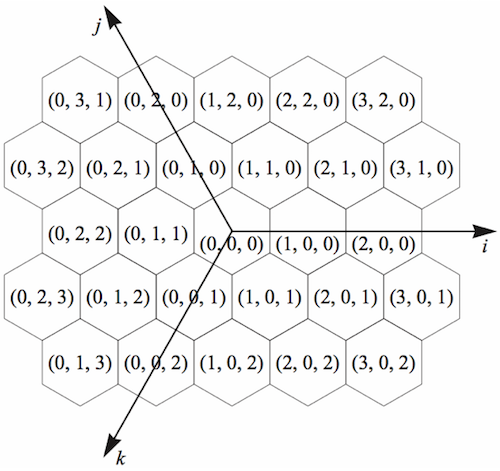
\includegraphics[width=15cm,height=12cm]{ijkp.png}
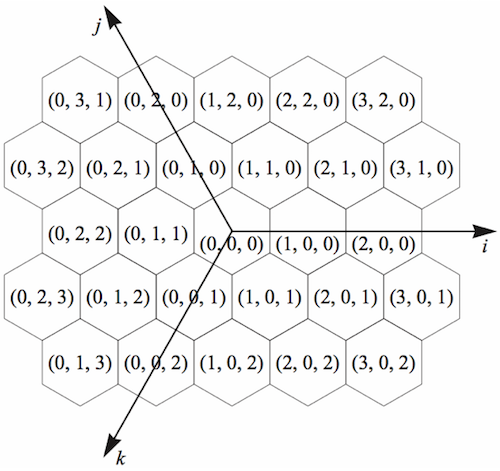
\includegraphics[scale=0.3]{ijkp.png}
\caption{One possible map example that using the \textit{ijk} coordinate system} % 标题
\end {figure}

% Notations
\subsubsection{Notations}
Here are all the notations and their meanings in this paper.
\begin{table}[h]
    \centering
    \caption{Notations used in model construction}
    \vspace{3pt}
    \begin{tabular}{>{\centering\arraybackslash}p{6em}>{\centering\arraybackslash}p{30em}}
        \toprule % 绘制第1条线
        Notation         & Meaning                                 \\
        \midrule % 绘制第2条线
        $M
        (i,t)$           & Location of the $i$-th drone
        \uppercase\expandafter{\romannumeral1} at time $t$         \\
        $R
        (j,t)$           & Location of the $j$-th drone
        \uppercase\expandafter{\romannumeral2} at time $t$         \\
        $h
        (x,y,z)$         & Elevation of the point $(x,y,z)$        \\
        $S
        (x,y,z)$         & Fire history of the point $(x,y,z)$
        in the passed $5$ years                                    \\
        $a_i
        (x,y,z)$         & Fire history of the point $(x,y,z)$
        in the $2020-i$-th year,
        $i\in [1,5] \cap \mathbb{N} $                              \\
        $F(x,y,z) $      & Vegetation and urbanizing
        condition of the point$(x,y,z)$                            \\
        $Str(i,x,y,z,t)$   & Signal strength of the
        $i$-th drone at point $(x,y,z)$ at time $t$                \\
        $E
        (x,y,z,N)$       & Supervisory density of
        the point $(x,y,z)$ when there are $N$ drones in the field \\
        $Slope
        (x,y,z)$         & Maximum slope of the point $(x,y,z)$    \\
        $\gamma$         & Factor related to the weight
        of slope in causing bushfire                               \\
        $\beta
        (x,y,z)$         & Weight of slope in causing bushfire     \\
        $\omega
        (x,y,z)$         & Decreasing rate of signal
        at point $(x,y,z)$                                         \\
        $\alpha$         & Factor related to the weight
        of elevation in causing bushfire                           \\
        $Chg
        (q,x,y,z)$       & Location of the $q$-th charging station \\
        $V_{\text{max}}$ & Maximum flying velocity of a drone      \\
        $N_{\text{SSA}}$ & Amount of drone
        \uppercase\expandafter{\romannumeral1}                     \\
        $N_{\text{rep}}$ & Amount of drones
        \uppercase\expandafter{\romannumeral2}                     \\
        $PF$             & Power consumption for a flying drone    \\
        $PH$             & Power consumption for a hovering drone  \\
        $t_{\text{fl}}
        (t,l)$           & Flight time of the $l$-th drone
        until time $t$                                             \\
        $t_{\text{hov}}
        (t,l)$           & Hovering time of the $l$-th drone
        until time $t$                                             \\
        $T$              & Duration of a day (i.e. $T=1440 \min$)  \\
        $t$              & Current time                            \\
        $Br$             & Total battery power of a drone          \\
        $Ini$            & Location of the EOC                     \\
        \bottomrule
    \end{tabular}
\end{table}
\section{Model Construction}
%%%%%%%%%%%%%%%%%%%%%%%%%%%%%%%%%%%%%%%
%% Model Construction
\subsection{Multi-factor Evaluating Model}
% M1
% 标题太长了 会改的
% 原文后面还有一小段短语 for Segmentation and Assessment of the Topography
In this section, we introduce a H3 and multi-factor evaluating model to data-orienting the topographic conditions of the state Victoria in Australia.

First, in order to simplify the question, we cover the state with hexagons in dense tiled layout. We consider that the valid zone of radio wave signal radiated by a UAV is a spherical area of radius 20 km, and the length of each side of hexagon is 1.22 km.

Next, we evaluated each segment from 4 dimensions, which are: density of forest coverage, elevation, slope and fire history. We consider the influence of the listed dimensions from two aspects: how dose it influence the possibility to catch fire for the area and how does it influence the propagation of radio wave signal. The mechanism and significance of these factors are discussed below.

\subsubsection{The Influence of Vegetation and Other Ground Facilities}
%%% M1F1
According to Dissing and Verbyla (2003) \cite{Dorte-lightning01}, thermal circulations triggered by differential heating among distinct types of vegetation results in a higher probability for a lighting strike to occur. But according to a later research based in the State of Victoria (Kilinc and Beringer 2006 \cite{Musa-lightning02}), vegetation type and density in Southern region of Australia have little impact on the occurrence rate of lightning. Mainly because of the homogeneity of forests.

On the other hand, the leafage has a significant impact on the reflection behavior of radio wave, which plays an important part in the propagation process. Different researches have been done to estimate the decreasing rate of radio wave in varies situations, the shared mechanism underneath is Fresnel's Law. We divided the surroundings into three categories: forests, plain, cities, then we estimated the decrease factor and valid zone for the radio signal distinctively.

Since the given signal's frequency ranges from 300 megahertz to 3,000 megahertz and from 30 megahertz to 300 megahertz, which are considerably high, so it is difficult for the signal to steer by high-rise structures, including tall buildings and mountains. When our drones are passing through the plain area, the the energy lose for the signal strengths is in the air, so the radius of the valid zone for the signal reaches it's maximum of 20km. When the drone is passing a urban area, high obstacles diminished the zone and the radius reaches it's minimum of 5km. When the drones are flying or hovering in forest region, two situations should be discussed separately, the ground signal from wearable devices on front-line personnel and the aerial signal from another drone. According to the data of the experiments done by Y.S. Meng.et.al (2010) \cite{Ng-vhf-radio}, when the signal is launched in woods, the signal strength decreases linearly with the frequency of radio wave, and distance (Y. S. Meng.et.al 2009 \cite{Ng-vhfuhf-ieee}).

According to their model, the foliage loss in forest region is defined by the equation below:
\begin{equation}\label{ldb}
    L({\rm dB})\cong 0.48 f^{0.43} d^{0.13}
\end{equation}

Considering the drone-to-drone signal propagation, we simply omit the influence of trees, for it is reasonable for flying vehicles to stay above the forests. According to Meng, the background noise is around -75 dBm, so we consider the signal to be undetectable if its strength is lower than -70 dBm. Which means that when the strength loss is over 18 dB, we consider this point to be inaccessible. Using Equation \eqref{ldb} and the data we have, we can verify the decreasing coefficient for different area as follow:
\begin{equation}\label{omega-function}
    \overline{\omega}
    (x,y,z)=
    \left\{
    \begin{aligned}
         & \overline{\omega}_{\text{city}}=0.25,  \\
         & \overline{\omega}_{\text{forest}}=0.5, \\
         & \overline{\omega}_{\text{plain}}=1
    \end{aligned}
    \right.
\end{equation}

\subsubsection{The Influence of Elevation and Slope}
%%% M1F2
As we mentioned above, the Mountains would worsen the signal, thus, it is natural to introduce an elevation factor $A$ here to evaluate the impact of elevation on causing bushfires.

Annual lightning strikes were so connected to local elevation and slope that many scholars have been using topographic methods to predict bush-fire in mountainous regions \cite{Jiao-wildfire-cn}. Previous research has shown that strike density has a great leap while the local elevation reaches 800 meters and increases linearly with elevation \cite{Musa-lightning02}, and it is more likely for a mountainous area to form strikes comparing to an area with only one high-rise peak \cite{Jiao-wildfire-cn}.


\subsubsection{The Influence of Fire History}
%%% M1F3
Burned area is more likely to be caught on fire in the future, according to Musa Kilinc and Jason Beringer \cite{Musa-lightning02}. Because ecological environment has been destroyed in the fire, which results in a low capability of local temperature and low capacity of water. None the less, the coked ground with dark shade will absorb more heat than green forests. All these traits formed a hot dry area which can be easily lighted by strikes.

\subsubsection{Functionizing the state of certain location}
%%% M1-Function
To describe a certain location $(x,y,z)$ in the \textit{ijk} coordinate system, we adopted a series of functions\dots

The elevation of the location is denoted by $h(x,y,z)$ , while its slope is denoted by $Slope(x,y,z)$, which means the maximum slope around one point:
\begin{equation}\label{slope}
    \begin{aligned}
        Slope(x,y,z)&=\max\left\{
            \frac{\lVert
                    h(x,y,z)-h(x+m,y+n,z+k)
                    \rVert}
            {\lvert m\rvert+\lvert n\rvert+\lvert k\rvert}
            \right\},\\
            & m,n,k\in\{-1, 0, 1\},
        \end{aligned}
    \end{equation}

Besides, The unit of $h(x,y,z)$ and $Slope(x,y,z)$ are both meters.
\\
The weight of $Slope(x,y,z)$ in causing bushfires is
\begin{equation}\label{weight of slope}
    \begin{aligned}
        \beta(x,y,z)&=\gamma\cdot \max\left\{
            \frac{
                Slope(x,y,z)-Slope(x+m,y+n,z+k)
                }
            {\lvert m\rvert+\lvert n\rvert+\lvert k\rvert}
            \right\},\\
            &\gamma\text{ is a constant, and } m,n,k\in\{-1, 0, 1\},
    \end{aligned}
\end{equation}

The vegetational and urbanizing condition $F(x,y,z)$ is defined as the following equation:
\begin{equation}\label{vegetation}%equ6
    F(x,y,z)=
    \left\{
    \begin{aligned}
         & 1,\qquad (x,y,z)\text{ locates in forests,} \\
         & 0,\qquad \text{otherwise.}
    \end{aligned}
    \right.
\end{equation}

The influence of fire history is quantified by bushfire frequency in the passed 5 years (i.e. 2016-2020) :%equ.7
\begin{equation}\label{Fire-history}
    \begin{aligned}
        S(x,y,z)=\sum_{i=1}^5 (1+\epsilon)^{\frac{1}{i}}\cdot a_i,\quad a_i=\frac{f_i}{23},
    \end{aligned}
\end{equation}
%!check
Here $f_i$ is the amount of fire cases in the $n-i$-th year.

Then we define a function $V(x,y,z)$ to represent how possible a point will catch fire. It is defined below :
\begin{equation}\label{PossibilityFire}
    \begin{aligned}
        V(x,y,z) =& V_1(x,y,z)\cdot V_2(x,y,z), \\
        \text{Note: }\quad V_1(x,y,z) &= [
            0.58 F(x,y,z)\\
           & +\alpha\left(
                h(x,y,z)-800
                 \right)\cdot
                 \beta\cdot u(h(x,y,z)-800)
            ], \\
        V_2(x,y,z) &=\left[
            1+\frac{\ln \left(1+S\left(x,y,z\right)\right)}{3}
            \right],
    \end{aligned}
\end{equation}

here $u(\delta)$ is the stair function:
\begin{equation}\label{Stair}%{equ.11}
    u(\delta)=
    \left\{
    \begin{aligned}
         & 1,\qquad \delta> 0,\\
         & 0,\qquad \delta\leq 0.
    \end{aligned}
    \right.
\end{equation}

\subsubsection{Future situation in a decade}
%%% M1-Predict
To predict the changing situation in the next decades, we reevaluate the area in the future with the multi-factor model above. Since we do not take extreme events into consideration (severe war, earthquake, tsunami, meteorolite, EI Nino etc.), the landscape and urban constructions will not change much in the next decade. The only changing factor is the fire history of on point, which was evaluated by Equation \ref{Fire-history}, and the fire “history” in future is represented by the possibility of that year to catch fires, and was described by the function below

%!!!!!!!equ10

here the threshold $867.35$ means that the possibility of catch fires is 95\% .


\subsection{Use Nervous System Model to find the best arrangement of UAVs}
% M2
Widespread bushfires in Australia are usually preceded by strong winds, a small-scale burning forests can evolve into destructive fires. So in other to minimize the damage caused by bushfires, it is reasonable to build up a monitoring and alarming system to supervise the region before any outbreaks. In this section, our group build up a model imitating the nervous system to sort out the best arrangement of UAVs.

In our model, drones with thermal imaging cameras and telemetry sensors (drone \uppercase\expandafter{\romannumeral1}) are send out to petrol around the state, detecting fire outbreaks and sending back images, they are working as sensors of a nervous system. While drones with radio repeaters (drone \uppercase\expandafter{\romannumeral2}) act like ganglion, they receive signals and send them out immediately, the command center is the brain in this system. Our goal is achieved by two steps. First, find the best routes for drones\uppercase\expandafter{\romannumeral1}. In order to react to fire out breaks timely, the monitoring system should

\begin{itemize}
    \item Cover the state with its valid zone,
    \item Pay closer attention to the points who have higher probability of catching fire.
\end{itemize}

To further the discussion, we have two new functions: first for signal strength, and second for average signal density of one point:
% equ. 19, 20
\begin{subequations}
    \begin{equation}
        Str(i,x,y,z,t)=u\left(8-\lVert (x,y,z)-M(i,t)\rVert\right),
    \end{equation}
    \begin{equation}
        E(x,y,z,N)=\sum_{i=1}^{N_{\text{SSA}}}\frac{1}{T}\int_{0}^{T}S(i,x,y,z,t)dt,
    \end{equation}
\end{subequations}

From the discussion in section 1, we construct the function \label{PossibilityFire} to evaluate how high the possibility is for a point to catch fire, and here we introduce a function $Judge(x, y,z)$ defined as $Judge(x,y,z)=\frac{\eta \cdot E}{V}-1$ to judge whether a point is safe enough, by safe enough we mean the possibility for any drone \uppercase\expandafter{\romannumeral1} to discover a outbreak immediately is high. Here we set the threshold to be 80 percent, thus $\lambda_{\text{safe}}=0.8$.

Second, we should link the sensors to the brain. As discussed in the section 1, we omit the signal loss caused by forests, but we take the influence of high buildings into consideration. So here we define two kinds of vectors $D_i(t)=[d_{ij}(t)]$ and $Q_j(t)=[b_{jk}(t)]$  to represent the signal path from sensors to the center. The vectors are defined as below

%equ 16
\begin{subequations}
    \begin{equation}
        d_{ij}(t)=\left\{
            \begin{aligned}
                &1, \quad \text{if } 0< \lVert M(i,t)-R(j,t)\rVert< 8,\\
                &0,\quad \text{otherwise},
            \end{aligned}
        \right.
    \end{equation}
    \begin{equation}
        b_{jk}(t)=\left\{
            \begin{aligned}
                &1, \quad \text{if } 0< \lVert R(k,t)-R(j,t)\rVert< 8,\\
                &0,\quad \text{otherwise},
            \end{aligned}
        \right.
    \end{equation}
\end{subequations}

 Here $i$ denotes the number of drone \uppercase\expandafter{\romannumeral1}s, while $j$ and $k$ denote the number of drone \uppercase\expandafter{\romannumeral2}s.

To guarantee that the command center can react to any out break in time, the signal paths should keep unimpeded at all time, then the variables are limited by the following inequality constraints under this requirement.

%equ.17
\begin{subequations}
    \begin{equation}
        \sum_{j=1}^{N_{\text{rep}}}d_{ij}\geq 1, \quad i=1,2,\cdots,N_{\text{SSA}}
    \end{equation}
    \begin{equation}
        \sum_{k=1}^{N_{\text{rep}}}b_{jk}\left\{
        \begin{aligned}
            \geq 1,& \qquad \text{if }\sum_{i=1}^{N_{\text{SSA}}} d_{ij}\geq 1,\\
            \geq 2,& \qquad \text{otherwise},
        \end{aligned}
        \right.
    \end{equation}
\end{subequations}

One last thing should be considered in this section, which is the recycle of drones. Under assumption 9 (see \ref{ampt09}), none of our drones would be allowed to go further than the distance they can get back to charging stations before they run out of buttery. This give the constraints below.

% equ. 18
\begin{subequations}
    \begin{equation}
        t_{\text{hov}}+t_{\text{fly}}=t-105n,
    \end{equation}
    \begin{equation*}
     \text{Denotion: }\\
        k(n, t_{\text{fly}}, t_{\text{hov}}) = n\cdot Br-PF\cdot t_{\text{fly}}-PH\cdot t_{\text{hov}},
    \end{equation*}
    \begin{equation}
        k(n, t_{\text{fly}}, t_{\text{hov}})
        \geq
        \frac{\min\left\{
            \lVert
                M(i,t)-Chg(q)
            \rVert ,q
            \right\}}{
                0.417\cdot V_{\text{max}}
                },\text{ for }t\text{ and }i,
    \end{equation}
\end{subequations}

Here $0.417$ is the transformation coefficient between real velocity and grid velocity, and $n$ shows how many times that $i$-th drone went back to any charging station.


\subsection{Model for Rapid Bushfire Response}
% M3
Once any fire is spotted, command center will respond to the situation immediately, making sure that the communication network build up by UAVs will available in as possible a short time as possible. As discussed in section 1, the signal from forward teams will be weaken by vegetation and elevation. So here we should reconsider the signal strength around the fire,

{equ.21}

then we recalculate the average signal density of one point depending on time,

{equ.22}

when the new signal density surpass the threshold we set, we regard this point to be accessible and hover the drones to hold the signal. The time interval between the moment fires have been spotted and the time the communication network has been build is the reacting time, and we want it to be as short as possible. Under these assumptions we can find out an efficient way to re-construct the distribution of drones.

% M4
\subsection{Model for Hovering Drones for Fires of Different Sizes on Different Terrains}
In the first model, we evaluated each hexagons from 4 aspects, and in the third model we considered the decreasing rate in different terrains, so in this model we combine this two models to sort out the best hovering positions for fires of different sizes on different terrains.

It is reasonable for us to assume that the forward teams will never go inside a burning forest, so the valid zone of radio signal only need to cover the premier of any fires. Since we want to keep the drones static to hold the signal path, and at the same time, we need them to come back when they are running out of buttery, so we arrange the drones as below:

\begin{itemize}
    \item We need drone \uppercase\expandafter{\romannumeral2}s to keep in touch with the front teams;
   \item We need drone \uppercase\expandafter{\romannumeral1}s to monitor and report data from wearable devices on front-line personnel;
    \item As long as there is a fire spotted, except the drones needed to build the communication net, other drones will go back to charge stations to stand by.
\end{itemize}

To satisfy these requirements we again recalculate the signal strength average signal density as below,

{equ.23}

    {equ.24}

because the drones are now static, the signal now is a constant as time changes.

We also need the forward drones to be connected to the command center. This restriction is described by the formulas below.

    {equ.16}

    {equ.17}


\section{Model Simulation}
%%%%%%%%%%%%%%%%%%%%%%%%%%%%%%%%%%%%%%%
%% Model Simulation


\subsection{Nervous System model for UAVs Monitoring System}
% S1


\subsubsection{Adapting for Future}
% 这里有点奇怪


\subsection{Modeling for Rapid Bushfire Response}
% S2


\subsection{Model for the hovering drones SSA and Radio Repeater}
% S3


\section{Sensitive Analysis}
%%%%%%%%%%%%%%%%%%%%%%%%%%%%%%%%%%%%%%%
%% Sensitive Analysis
\subsection{ensitivity of parameters}
abaaba
\subsection{Robusticity of the models}

\section{Strength and Weakness}
%%%%%%%%%%%%%%%%%%%%%%%%%%%%%%%%%%%%%%%
%% Strength and Weakness
\subsection{Strength}


\subsection{Weakness}


\section{Conclusion}
%%%%%%%%%%%%%%%%%%%%%%%%%%%%%%%%%%%%%%%
%% Conclusion
We build a.....interesting findings:

\begin{itemize}
    \item aaaaaaa
    \item aaaaaaa
\end{itemize}

\newpage
\section*{References}\addcontentsline{toc}{section}{References}
%%%%%%%%%%%%%%%%%%%%%%%%%%参考文献%%%%%%%%%%%%%%%%%%%%%%%%%%
% 因为不输出此部分到目录 \addcontentsline{}{}{}是添加此标题到目录
\fancyhf{}
\fancyhead[R]{ }
\fancyhead[L]{ }
\bibliography{books}
\Large
\bibliographystyle{IEEEtran}
\newpage

\section*{Appendices}\addcontentsline{toc}{section}{Appendices for Code and Data}
%%%%%%%%%%%%%%%%%%%%%%%%%%附录%%%%%%%%%%%%%%%%%%%%%%%%%%
\fontsize{13pt}{12.5pt}\selectfont
foooo
\vspace{7pt}
\subsection*{Appendices A}
fooooo

\end{document}